\section{Auswertung}
\label{sec:Auswertung}
\subsection{Bestimmung des Materials der Stäbe}
\label{sec:Material}
Mit den aus \ref{sec:Stäbe} bekannten Abmessungen ergeben sich die Dichten $\rho$ der Stäbe mittels
\begin{equation}
  \rho = \frac{m}{V} = \frac{m}{Al}
\end{equation}
und
\begin{equation}
  A_r = \pi r^2
\end{equation}
bzw
\begin{equation}
  A_q = a^2
\end{equation}
zu $\rho_r =8397 \frac{kg}{m^3}$  bzw. $\rho_q = 8373 \frac{kg}{m^3}$. Messing CuZnPb3 beispielsweise besitzt eine Dichte von $\rho_{Messing} = 8.47 \cdot 10^9 \frac{kg}{m^3}$ und einem Elastizitätsmodul von $E_{Messing} = 9.7 \cdot 10^10 {N}{m^2}$ \cite{DKI}. Es wird somit von Messingstäben ausgegangen und als vergleichender Theoriewert $E_{Messing}$ hinzugezogen. Auf qualitativen Vergleich wird jedoch verzichtet, da Messing als Legierung je nach Ausführung enorme Unterschiede in seiner Beschaffenheit aufweisen kann.
\subsection{Einseitige Einspannung}
\label{sec:Einseitig}

\begin{table}
  \centering
  \caption{Auslenkung des runden Stabes bei einseitiger Einspannung}
  \label{tab:einseitig-r}
  \sisetup{round-mode = places , round-precision = 3}
  \begin{tabular}{S S S S}
    \toprule
    {$x/cm$} & {$D_o/mm$} & {$D_m /mm$} & {$\Delta D /mm$}\\
    \midrule
    3.000000000000000000e+0 & 0.000000000000000000e+00 & 0.05000000000000000278e-0 & 0.05000000000000000278e-0\\
    4.000000000000000000e+0 & 0.000000000000000000e+00 & 0.04200000000000000261e-0 & 0.04200000000000000261e-0\\
    5.000000000000000000e+0 & 0.04750000000000000056e-0 & 0.05619999999999999996e-0 & 0.008699999999999999400e-0\\
    6.000000000000000000e+0 & 0.05500000000000000028e-0 & 0.1100000000000000006e-0 & 0.05500000000000000028e-0\\
    7.000000000000000000e+0 & 0.06500000000000000222e-0 & 0.1680000000000000104e-0 & 0.1030000000000000082e-0\\
    8.000000000000000000e+0 & 0.1000000000000000056e-0  & 0.2250000000000000056e-0 & 0.1250000000000000000e-0\\
    9.000000000000000000e+0 & 0.1549999999999999989e-0 & 0.2909999999999999809e-0 & 0.1359999999999999820e-0\\
    10.00000000000000000e+0 & 0.1799999999999999933e-0 & 0.3549999999999999822e-0 & 0.1749999999999999889e-0\\
    11.00000000000000000e+0 & 0.2179999999999999993e-0 & 0.4199999999999999845e-0 & 0.2019999999999999851e-0\\
    12.00000000000000000e+0 & 0.2780000000000000249e-0 & 0.4899999999999999911e-0 & 0.2119999999999999662e-0\\
    13.00000000000000000e+0 & 0.3175000000000000044e-0 & 0.5819999999999999618e-0 & 0.2644999999999999574e-0\\
    14.00000000000000000e+0 & 0.3300000000000000155e-0 & 0.6600000000000000311e-0 & 0.3300000000000000155e-0\\
    15.00000000000000000e+0 & 0.3699999999999999956e-0 & 0.7099999999999999645e-0 & 0.3399999999999999689e-0\\
    16.00000000000000000e+0 & 0.4249999999999999889e-0 & 0.8000000000000000444e-0 & 0.3750000000000000555e-0\\
    17.00000000000000000e+0 & 0.4899999999999999911e-0 & 0.9000000000000000222e-0 & 0.4100000000000000311e-0\\
    18.00000000000000000e+0 & 0.5999999999999999778e-0 & 1.040000000000000036e+00 & 0.4400000000000000577e-0\\
    19.00000000000000000e+0 & 0.6899999999999999467e-0 & 1.165000000000000036e+00 & 0.4750000000000000888e-0\\
    20.00000000000000000e+0 & 0.7349999999999999867e-0 & 1.268000000000000016e+00 & 0.5330000000000000293e-0\\
    21.00000000000000000e+0 & 0.8100000000000000533e-0 & 1.381000000000000005e+00 & 0.5709999999999999520e-0\\
    22.00000000000000000e+0 & 0.9280000000000000471e-0 & 1.550000000000000044e+00 & 0.6219999999999999973e-0\\
    23.00000000000000000e+0 & 1.000000000000000000e+00 & 1.705000000000000071e+00 & 0.7050000000000000711e-0\\
    24.00000000000000000e+0 & 1.070000000000000062e+00 & 1.784999999999999920e+00 & 0.7149999999999998579e-0\\
    25.00000000000000000e+0 & 1.129999999999999893e+00 & 1.919999999999999929e+00 & 0.7900000000000000355e-0\\
    26.00000000000000000e+0 & 1.237500000000000044e+00 & 2.250000000000000000e+00 & 1.012499999999999956e+00\\
    27.00000000000000000e+0 & 1.314999999999999947e+00 & 2.169999999999999929e+00 & 0.8549999999999999822e-0\\
    28.00000000000000000e+0 & 1.385000000000000009e+00 & 2.270000000000000018e+00 & 0.8850000000000000089e-0\\
    29.00000000000000000e+0 & 1.449999999999999956e+00 & 2.399999999999999911e+00 & 0.9499999999999999556e-0\\
    30.00000000000000000e+0 & 1.540000000000000036e+00 & 2.555000000000000160e+00 & 1.015000000000000124e+00\\
    31.00000000000000000e+0 & 1.622999999999999998e+00 & 2.750000000000000000e+00 & 1.127000000000000002e+00\\
    32.00000000000000000e+0 & 1.449999999999999956e+00 & 2.825000000000000178e+00 & 1.375000000000000222e+00\\
    33.00000000000000000e+0 & 1.792000000000000037e+00 & 2.959999999999999964e+00 & 1.167999999999999927e+00\\
    34.00000000000000000e+0 & 1.860000000000000098e+00 & 3.084999999999999964e+00 & 1.224999999999999867e+00\\
    35.00000000000000000e+0 & 1.918                    & 3.250000000000000000e+00 & 1.332000000000000073e+00\\
    36.00000000000000000e+0 & 2.01                     & 3.359999999999999876e+00 & 1.350000000000000089e+00\\
    37.00000000000000000e+0 & 2.060000000000000053e+00 & 3.500000000000000000e+00 & 1.439999999999999947e+00\\
    38.00000000000000000e+0 & 2.085                    & 3.620000000000000107e+00 & 1.535000000000000142e+00\\
    39.00000000000000000e+0 & 2.19e+00                 & 3.785000000000000142e+00 & 1.595000000000000195e+00\\
    40.00000000000000000e+0 & 2.270000000000000018e+00 & 3.904999999999999805e+00 & 1.634999999999999787e+00\\
    41.00000000000000000e+0 & 2.350000000000000089e+00 & 4.044999999999999929e+00 & 1.694999999999999840e+00\\
    42.00000000000000000e+0 & 2.635e+00                & 4.174999999999999822e+00 & 1.540000000000000036e+00\\
    43.00000000000000000e+0 & 2.540000000000000036e+00 & 4.339999999999999858e+00 & 1.799999999999999822e+00\\
    44.00000000000000000e+0 & 2.625000000000000000e+00 & 4.549999999999999822e+00 & 1.924999999999999822e+00\\
    45.00000000000000000e+0 & 2.735                    & 4.629999999999999893e+00 & 1.895000000000000018e+00\\
    46.00000000000000000e+0 & 2.82                     & 4.834999999999999964e+00 & 2.015000000000000124e+00\\
    47.00000000000000000e+0 & 2.910000000000000142e+00 & 5.019999999999999574e+00 & 2.109999999999999432e+00\\
    48.00000000000000000e+0 & 2.985                    & 5.184999999999999609e+00 & 2.199999999999999734e+00\\
    49.00000000000000000e+0 & 3.120000000000000107e+00 & 5.290000000000000036e+00 & 2.169999999999999929e+00\\
    \bottomrule
  \end{tabular}
\end{table}

\begin{table}
  \centering
  \caption{Auslenkung des eckigen Stabes bei einseitiger Einspannung}
  \label{tab:einseitig-q}
  \sisetup{round-mode = places , round-precision = 3}
  \begin{tabular}{S S S S}
    \toprule
    {$x/cm$} & {$D_o/mm$} & {$D_m /mm$} & {$\Delta D /mm$}\\
    \midrule
    3.000000000000000000e+00 & 0.000000000000000000e+00 & 0.02000000000000000042e-0 & 0.02000000000000000042e-0\\
    5.000000000000000000e+00 & -0.04000000000000000083e-0 & -0.02000000000000000042e-0 & 0.02000000000000000042e-0\\
    7.000000000000000000e+00 & -0.07000000000000000666e-0 & 0.08000000000000000167e-0 & 0.1500000000000000222e-0\\
    9.000000000000000000e+00 & -0.05500000000000000028e-0 & 0.1900000000000000022e-0 & 0.2449999999999999956e-0\\
    11.00000000000000000e+0 & -0.01000000000000000021e-0 & 0.3300000000000000155e-0 & 0.3400000000000000244e-0\\
    13.00000000000000000e+0 & 0.02000000000000000042e-0 & 0.5150000000000000133e-0 & 0.4949999999999999956e-0\\
    15.00000000000000000e+0 & .05999999999999999778e-0 & 0.6680000000000000382e-0 & 0.6080000000000000959e-0\\
    17.00000000000000000e+0 & 0.1199999999999999956e-0 & 0.9120000000000000329e-0 & 0.7920000000000000373e-0\\
    19.00000000000000000e+0 & 0.2949999999999999845e-0 & 1.270000000000000018e+00 & 0.9750000000000000888e-0\\
    21.00000000000000000e+0 & 0.4299999999999999933e-0 & 1.580000000000000071e+00 & 1.150000000000000133e+00\\
    23.00000000000000000e+0 & 0.5699999999999999512e-0 & 1.899999999999999911e+00 & 1.330000000000000071e+00\\
    25.00000000000000000e+0 & 0.6830000000000000515e-0 & 2.205000000000000071e+00 & 1.522000000000000020e+00\\
    27.00000000000000000e+0 & 0.7950000000000000400e-0 & 2.555000000000000160e+00 & 1.760000000000000231e+00\\
    29.00000000000000000e+0 & 0.9200000000000000400e-0 & 2.915000000000000036e+00 & 1.995000000000000107e+00\\
    31.00000000000000000e+0 & 1.070000000000000062e+00 & 3.310000000000000053e+00 & 2.240000000000000213e+00\\
    33.00000000000000000e+0 & 1.235000000000000098e+00 & 3.714999999999999858e+00 & 2.479999999999999538e+00\\
    35.00000000000000000e+0 & 1.387999999999999901e+00 & 4.125000000000000000e+00 & 2.737000000000000099e+00\\
    37.00000000000000000e+0 & 1.495000000000000107e+00 & 4.509999999999999787e+00 & 3.014999999999999680e+00\\
    39.00000000000000000e+0 & 1.705000000000000071e+00 & 4.974999999999999645e+00 & 3.269999999999999574e+00\\
    41.00000000000000000e+0 & 1.879999999999999893e+00 & 5.419999999999999929e+00 & 3.540000000000000036e+00\\
    43.00000000000000000e+0 & 2.009999999999999787e+00 & 5.879999999999999893e+00 & 3.870000000000000107e+00\\
    45.00000000000000000e+0 & 2.169999999999999929e+00 & 6.309999999999999609e+00 & 4.139999999999999680e+00\\
    47.00000000000000000e+0 & 2.365000000000000213e+00 & 6.820000000000000284e+00 & 4.455000000000000071e+00\\
    49.00000000000000000e+0 & 2.595000000000000195e+00 & 7.250000000000000000e+00 & 4.654999999999999361e+00\\
    \bottomrule
  \end{tabular}
\end{table}
\FloatBarrier

Für den runden Stab wurde eine Belastungsmasse von $m_1 = 238.9g$ gewählt, für den eckigen $m_2 = 767.5g$. Ihre Auslenkungen sind in den Tabellen \ref{tab:einseitig-r} und \ref{tab: einseitig-q} aufgelistet. Hierbei bezeichnet $x$ die Position auf dem Stab (Einspannung bei $x = 0$). $D_0$ die Auslenkung im unbelasteten Zustand, $ D_m$ die Auslenkung im belasteten Zustand und $\Delta D$ ihre Differenzen, also die Auslenkung durch die Belastung. Graphisch dargestellt sind die Werte in Abb.\ref{fig:Reihe1} bzw. Abb.\ref{fig:Reihe2}.

\begin{figure}
  \centering
  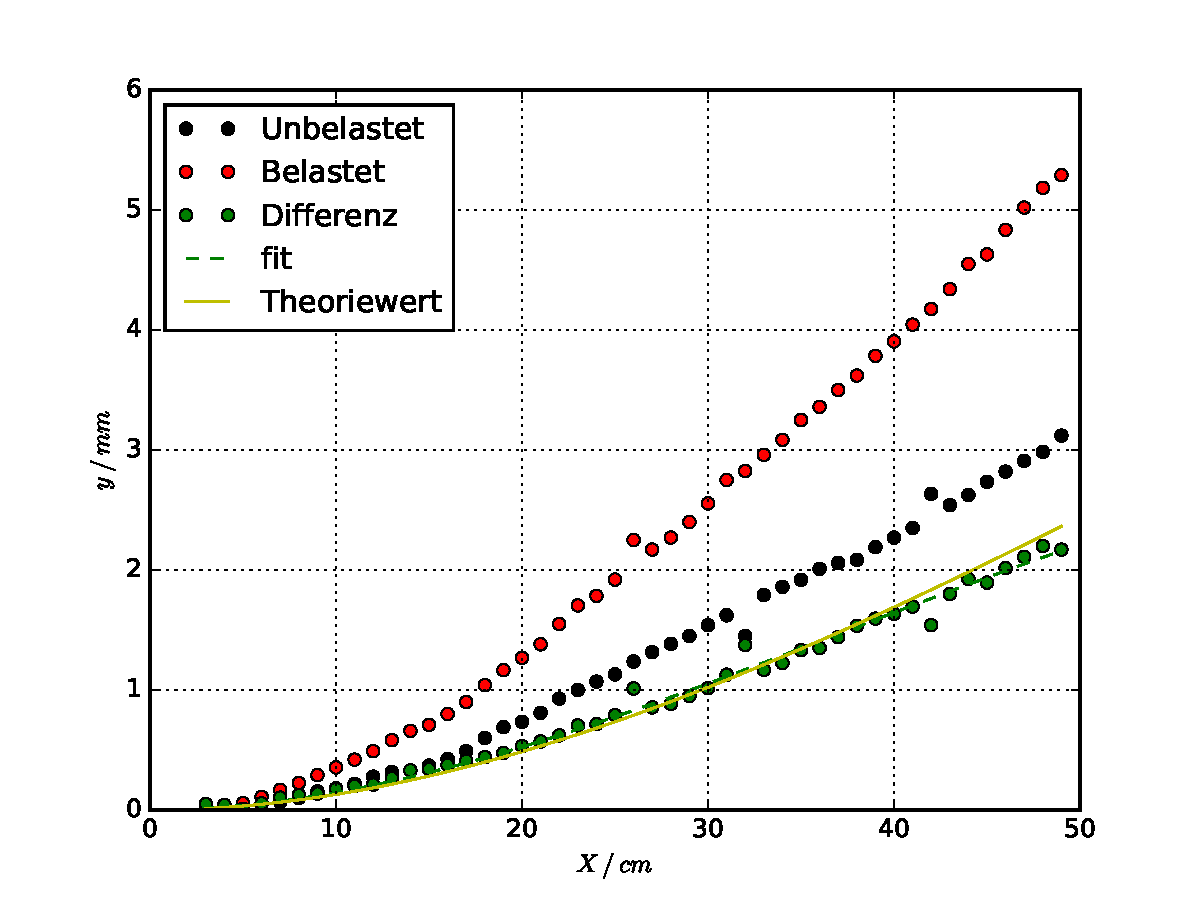
\includegraphics[width = \textwidth]{./Plots/Reihe1.pdf}
  \caption{Auslenkung des runden Stabes, verglichen mit dem Theoriewert}
  \label{fig:Reihe1}
\end{figure}

\begin{figure}
  \centering
  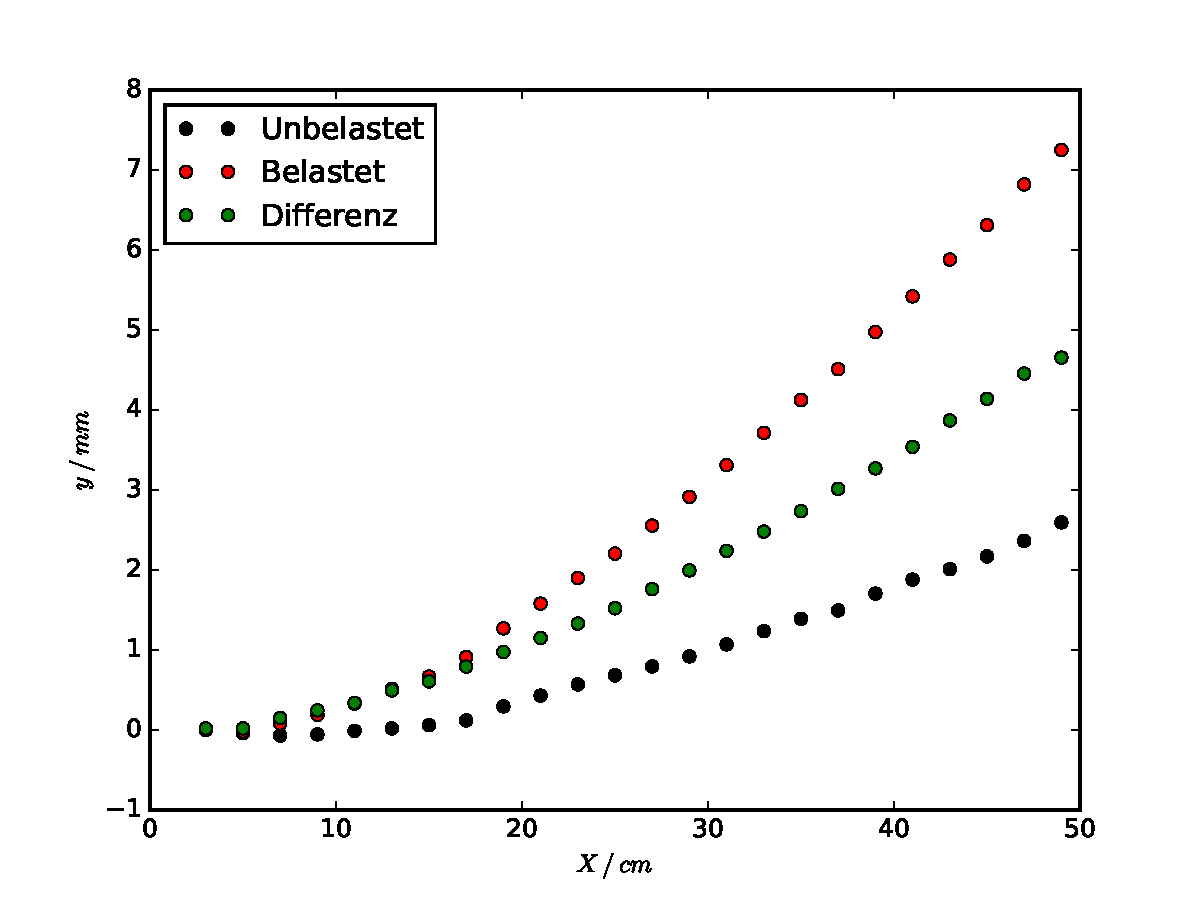
\includegraphics[width = \textwidth]{./Plots/Reihe2.pdf}
  \caption{Auslenkung des eckigen Stabes, verglichen mit dem Theoriewert}
  \label{fig:Reihe2}
\end{figure}

Die Flächenträgheitsmomente der Stäbe ergeben sich über \eqref{eqn:I} zu
\begin{equation}
  I_r = \frac{\pi}{64}d^4 = 4.9e-10 m^4
\end{equation}
bzw.
\begin{equation}
  I_q = \frac{a^4}{12} = 8.3e-10 m^4
\end{equation}

Mittels dieser Flächenträgheitsmomente und der Auslenkung der Stäbe lässt sich durch \eqref{eqn:D1} der Elastizitätsmodul bestimmen (Tabellen \ref{tab:Er} und \ref{tab:Eq}). Hierraus ergeben sich im Mittel

\begin{equation*}
  E_r = \left(9.76e9 \pm 4.3e9 \right) \frac{N}{m^2}
\end{equation*}
und
\begin{equation*}
  E_q = \left(1.35e10 \pm 6.1 e9 \right) \frac{N}{m^2}.
\end{equation*}

\begin{table}
  \centering
  \caption{$E_r$ berechnet aus $x$}
  \label{tab:Er}
  \sisetup{round-mode = places , round-precision = 2}
  \begin{tabular}{S S}
    \toprule
    {$x/cm$} & {$E_r / \frac{N}{m^2}$}\\
    \midrule
    3.000000000000000000e+00 & 2.432092196938775852e+07\\
    4.000000000000000000e+00 & 5.116917609329446405e+07\\
    5.000000000000000000e+00 & 3.836837394440537095e+08\\
    6.000000000000000000e+00 & 8.687441153988867998e+07\\
    7.000000000000000000e+00 & 6.276169733009708673e+07\\
    8.000000000000000000e+00 & 6.713881782857143879e+07\\
    9.000000000000000000e+00 & 7.762501448454383016e+07\\
    10.00000000000000000e+0 & 7.402069241982510686e+07\\
    11.00000000000000000e+0 & 7.711597506819559634e+07\\
    12.00000000000000000e+0 & 8.690394559106662869e+07\\
    13.00000000000000000e+0 & 8.123805974499444664e+07\\
    14.00000000000000000e+0 & 7.504283363636365533e+07\\
    15.00000000000000000e+0 & 8.308487788865548372e+07\\
    16.00000000000000000e+0 & 8.516494419591836631e+07\\
    17.00000000000000000e+0 & 8.737399755724242330e+07\\
    18.00000000000000000e+0 & 9.068984177643781900e+07\\
    19.00000000000000000e+0 & 9.299504283673468232e+07\\
    20.00000000000000000e+0 & 9.123058352797029912e+07\\
    21.00000000000000000e+0 & 9.327235468476358056e+07\\
    22.00000000000000000e+0 & 9.335322023426735401e+07\\
    23.00000000000000000e+0 & 8.942224613764655590e+07\\
    24.00000000000000000e+0 & 9.536317940345370770e+07\\
    25.00000000000000000e+0 & 9.302137892340481281e+07\\
    26.00000000000000000e+0 & 7.796992481934997439e+07\\
    27.00000000000000000e+0 & 9.889224443071967363e+07\\
    28.00000000000000000e+0 & 1.020418833898305297e+08\\
    29.00000000000000000e+0 & 1.012656415150375962e+08\\
    30.00000000000000000e+0 & 1.007231172715391666e+08\\
    31.00000000000000000e+0 & 9.618198553546531498e+07\\
    32.00000000000000000e+0 & 8.340871095807048678e+07\\
    33.00000000000000000e+0 & 1.036804972275126129e+08\\
    34.00000000000000000e+0 & 1.041859954335693866e+08\\
    35.00000000000000000e+0 & 1.008027519707207233e+08\\
    36.00000000000000000e+0 & 1.044580011428571343e+08\\
    37.00000000000000000e+0 & 1.026876175584608912e+08\\
    38.00000000000000000e+0 & 1.008599908621950448e+08\\
    39.00000000000000000e+0 & 1.014816731882157475e+08\\
    40.00000000000000000e+0 & 1.033608163265306354e+08\\
    41.00000000000000000e+0 & 1.039588796306664497e+08\\
    42.00000000000000000e+0 & 1.191588212337662280e+08\\
    43.00000000000000000e+0 & 1.060405572202381045e+08\\
    44.00000000000000000e+0 & 1.030185833702623993e+08\\
    45.00000000000000000e+0 & 1.086085022683215886e+08\\
    46.00000000000000000e+0 & 1.058934176441991478e+08\\
    47.00000000000000000e+0 & 1.047357177137537748e+08\\
    48.00000000000000000e+0 & 1.039362329053803682e+08\\
    49.00000000000000000e+0 & 1.089274183064516187e+08\\

    \bottomrule
  \end{tabular}
\end{table}

\begin{table}
  \centering
  \caption{$E_q$ berechnet aus $x$}
  \label{tab:Eq}
  \sisetup{round-mode = places , round-precision = 2}
  \begin{tabular}{S S}
    \toprule
    {$x/cm$} & {$E_q/ \frac{N}{m^2}$}\\
    \midrule
    3.000000000000000000e+00 & 1.204214435240963846e+08\\
    5.000000000000000000e+00 & 3.307243034638555050e+08\\
    7.000000000000000000e+00 & 8.544152138554215431e+07\\
    9.000000000000000000e+00 & 8.547381601917876303e+07\\
    11.00000000000000000e+0 & 9.093084076009921730e+07\\
    13.00000000000000000e+0 & 8.620173868200075626e+07\\
    15.00000000000000000e+0 & 9.231684034658369422e+07\\
    17.00000000000000000e+0 & 8.992455851816356182e+07\\
    19.00000000000000000e+0 & 9.012525593141797185e+07\\
    21.00000000000000000e+0 & 9.218407924305915833e+07\\
    23.00000000000000000e+0 & 9.441081186022284627e+07\\
    25.00000000000000000e+0 & 9.623102503641371429e+07\\
    27.00000000000000000e+0 & 9.581297827389101684e+07\\
    29.00000000000000000e+0 & 9.623833302382460237e+07\\
    31.00000000000000000e+0 & 9.664506589527754486e+07\\
    33.00000000000000000e+0 & 9.759140768922466040e+07\\
    35.00000000000000000e+0 & 9.811769616830490530e+07\\
    37.00000000000000000e+0 & 9.816806211412814260e+07\\
    39.00000000000000000e+0 & 9.915591415662653744e+07\\
    41.00000000000000000e+0 & 9.979236161170102656e+07\\
    43.00000000000000000e+0 & 9.896111094377507269e+07\\
    45.00000000000000000e+0 & 9.983354750523835421e+07\\
    47.00000000000000000e+0 & 9.970517434384000301e+07\\
    49.00000000000000000e+0 & 1.021555153772986829e+08\\

    \bottomrule
  \end{tabular}
\end{table}

\subsection{Beidseitige Auflage}
\label{sec:Beidseitig}

\begin{table}
  \centering
  \caption{Auslenkung des beidseitig aufgelegten runden Stabes}
  \label{tab:Erb}
  \sisetup{round-mode = places , round-precision = 2}
  \begin{tabular}{S S S S}
    \toprule
    {$x/cm$} & {$D_0 /mm$} & {$D_m / mm$} & {$\Delta D /mm$}\\
    \midrule
    3.000000000000000000e+00 & 0.02999999999999999889e-0 & 0.5649999999999999467e-0 & 0.5349999999999999201e-0\\
    5.000000000000000000e+00 & -0.04000000000000000083e-0 & 0.8649999999999999911e-0 & 0.9050000000000000266e-0\\
    7.000000000000000000e+00 & -0.1000000000000000056e-0 & 1.175000000000000044e+00 & 1.275000000000000133e+00\\
    9.000000000000000000e+00 & -0.1499999999999999944e-0 & 1.495000000000000107e+00 & 1.645000000000000018e+00\\
    11.00000000000000000e+0 & -0.1650000000000000078e-0 & 1.379999999999999893e+00 & 1.544999999999999929e+00\\
    13.00000000000000000e+0 & -0.2250000000000000056e-0 & 2.040000000000000036e+00 & 2.265000000000000124e+00\\
    15.00000000000000000e+0 & -0.3200000000000000067e-0 & 2.270000000000000018e+00 & 2.589999999999999858e+00\\
    17.00000000000000000e+0 & -0.3400000000000000244e-0 & 2.520000000000000018e+00 & 2.859999999999999876e+00\\
    19.00000000000000000e+0 & -0.2999999999999999889e-0 & 2.774999999999999911e+00 & 3.074999999999999734e+00\\
    21.00000000000000000e+0 & -0.3400000000000000244e-0 & 2.950000000000000178e+00 & 3.290000000000000036e+00\\
    23.00000000000000000e+0 & -0.3099999999999999978e-0 & 3.104999999999999982e+00 & 3.415000000000000036e+00\\
    25.00000000000000000e+0 & -0.3499999999999999778e-0 & 3.200000000000000178e+00 & 3.550000000000000266e+00\\
    30.00000000000000000e+0 & 0.7049999999999999600e-0 & 3.600000000000000089e+00 & 2.895000000000000018e+00\\
    32.00000000000000000e+0 & 0.6099999999999999867e-0 & 3.479999999999999982e+00 & 2.870000000000000107e+00\\
    34.00000000000000000e+0 & 0.5699999999999999512e-0 & 3.370000000000000107e+00 & 2.800000000000000266e+00\\
    36.00000000000000000e+0 & 0.5200000000000000178e-0 & 3.180000000000000160e+00 & 2.660000000000000142e+00\\
    38.00000000000000000e+0 & 0.4849999999999999867e-0 & 2.959999999999999964e+00 & 2.475000000000000089e+00\\
    40.00000000000000000e+0 & 0.4299999999999999933e-0 & 2.714999999999999858e+00 & 2.284999999999999698e+00\\
    42.00000000000000000e+0 & 0.3850000000000000089e-0 & 2.439999999999999947e+00 & 2.054999999999999716e+00\\
    44.00000000000000000e+0 & 0.3599999999999999867e-0 & 2.157500000000000195e+00 & 1.797500000000000320e+00\\
    46.00000000000000000e+0 & 0.2999999999999999889e-0 & 1.787500000000000089e+00 & 1.487500000000000044e+00\\
    48.00000000000000000e+0 & 0.2200000000000000011e-0 & 1.419999999999999929e+00 & 1.199999999999999956e+00\\
    50.00000000000000000e+0 & 0.1600000000000000033e-0 & 1.030000000000000027e+00 & 0.8699999999999999956e-0\\
    52.00000000000000000e+0 & 0.9800000000000000377e-0 & 0.6149999999999999911e-0 & 0.5170000000000000151e-0\\
    54.00000000000000000e+0 & 0.000000000000000000e+00 & 0.1900000000000000022e-0 & 0.1900000000000000022e-0\\
    \bottomrule
  \end{tabular}
\end{table}

In diesem Versuchsteil ist die Belastung $m_3 = 4722.5g$. Die Auslenkungen des Stabes sind Tabelle \ref{tab:beidseitig} zu entnehmen. Die Berrechnung von $E_r$ erfolgt diesmal durch \eqref{eqn:D2} ($x<27cm$) und \eqref{D3} ($x>27cm$). Ihre Ergebnisse lassen sich Tabelle \ref{tab:Erb} entnehmen. Hierbei ergibt sich der mittlere Elastizitätsmodul der beiden Seiten links ($x<27cm$) und rechts ($x>27cm$) zu
\begin{equation*}
  E_{links} = \left(1.07e10 \pm 8e8 \right)\frac{N}{m^2}
\end{equation*}
und
\begin{equation*}
  E_{rechts} = \left(1.587e10 \pm 6e7 \right) \frac{N}{m^2}
\end{equation*}

\begin{table}
  \centering
  \caption{$E_{r}$ berechnet aus $x$}
  \label{tab:Erb}
  \sisetup{round-mode = places , round-precision = 2}
  \begin{tabular}{S S}
    \toprule
    {$x/cm$} & {$E_r/\frac{N}{m^2}$}\\
    \midrule
    3.000000000000000000e+00 & 1.091563332642928660e+08\\
    5.000000000000000000e+00 & 1.068516625896733105e+08\\
    7.000000000000000000e+00 & 1.051430644826680869e+08\\
    9.000000000000000000e+00 & 1.033984258367385417e+08\\
    11.00000000000000000e+0 & 1.323117016126535833e+08\\
    13.00000000000000000e+0 & 1.044912702761775404e+08\\
    15.00000000000000000e+0 & 1.028824978931304514e+08\\
    17.00000000000000000e+0 & 1.025951820224975795e+08\\
    19.00000000000000000e+0 & 1.031428275735751539e+08\\
    21.00000000000000000e+0 & 1.025268713210350424e+08\\
    23.00000000000000000e+0 & 1.035114701746776551e+08\\
    25.00000000000000000e+0 & 1.029072679660552442e+08\\
    30.00000000000000000e+0 & 1.289862189238956422e+08\\
    32.00000000000000000e+0 & 1.280676701165902168e+08\\
    34.00000000000000000e+0 & 1.274540919390886575e+08\\
    36.00000000000000000e+0 & 1.284755721351069808e+08\\
    38.00000000000000000e+0 & 1.303244816543946117e+08\\
    40.00000000000000000e+0 & 1.311482947857238948e+08\\
    42.00000000000000000e+0 & 1.330829644096574336e+08\\
    44.00000000000000000e+0 & 1.359478122026320100e+08\\
    46.00000000000000000e+0 & 1.429876576892364025e+08\\
    48.00000000000000000e+0 & 1.490396020896440744e+08\\
    50.00000000000000000e+0 & 1.646029000332620740e+08\\
    52.00000000000000000e+0 & 2.053062434952365458e+08\\
    54.00000000000000000e+0 & 3.581164346951395273e+08\\

    \bottomrule
  \end{tabular}
\end{table}

\begin{figure}
  \centering
  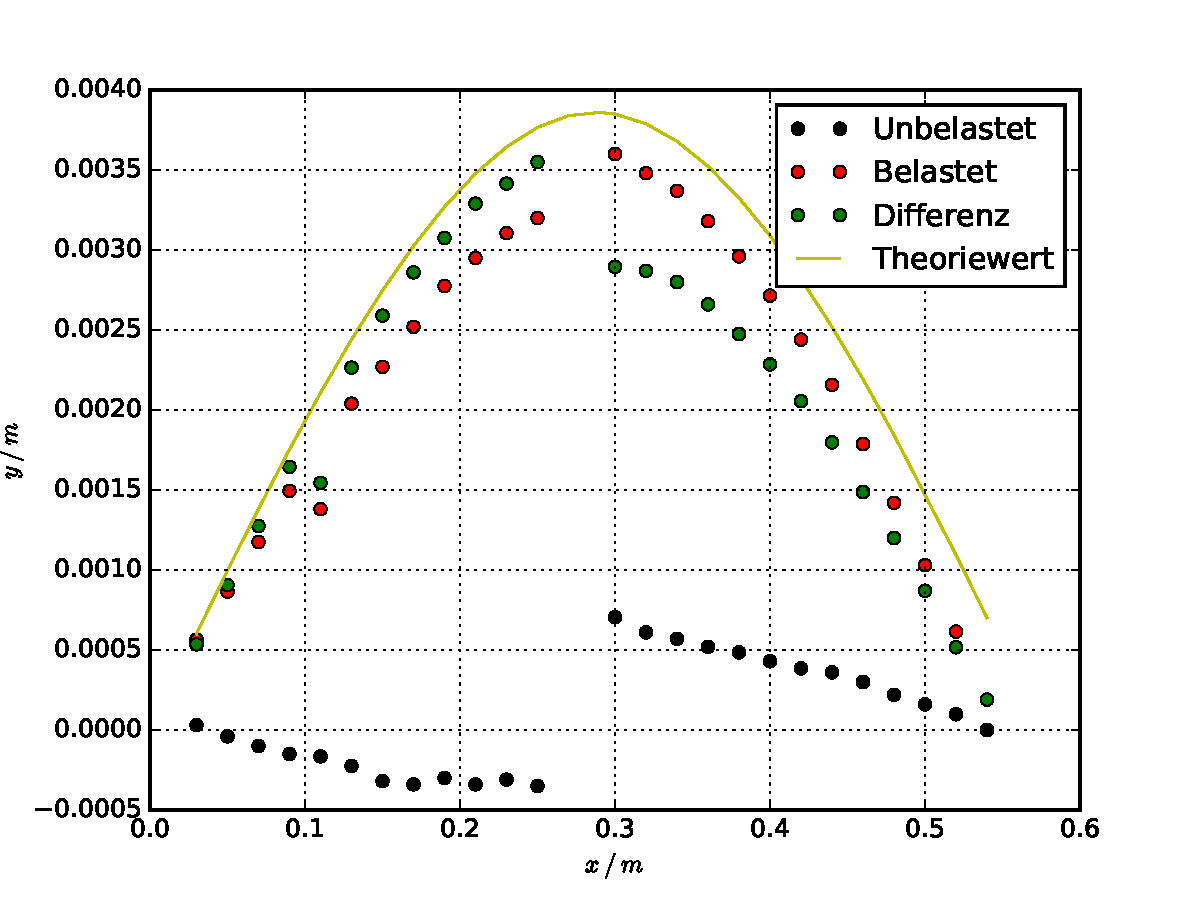
\includegraphics[width = \textwidth]{./Plots/Reihe3.pdf}
  \caption{Auslenkung des runden Stabes bei beidseitiger Auflage, verglichen mit dem Theoriewert}
  \label{fig:Reihe2}
\end{figure}
